\section{Problemas afrontados}

Una incorrecta elección de $R_t$ y $C_t$ para el TL494 fuera de los valores recomendados por el fabricante generaba variaciones muy grandes de la frecuencia de conmutación, 
lo cual causaba inestabilidad en la tensión de salida. 
Utilizando valores recomendados para ambos componentes se logró que la frecuencia posea una gran estabilidad.

Dado que la carga que genera el convertidor sobre el TL494 es muy alta, sin una etapa de ganancia de corriente, la forma de onda PWM 
se distorsionaba y disminuía notablemente su amplitud, lo que causaba que los MOSFETs no se saturaran y aumentaran demasiado su temperatura.
Los resultados obtenidos con la inclusión de esta etapa fueron una mejora en la forma de onda de la señal PWM y un incremento notorio en su amplitud.
Sin embargo, actualmente su amplitud disminuye al aumentar el ciclo de trabajo.

Al realizar las mediciones de tensión se evidenció un problema con la tierra de la PCB. 
La fuente regulable de 36V eleva notablemente su corriente entregada al circuito 
cuando se conecta la tierra de la punta del osciloscopio en ciertos puntos de la placa. 
Estas mediciones fueron tomadas estableciendo en la fuente un correcto límite de corriente. 
Además, en otros puntos como el transformador de potencia disminuye la tensión entregada por la fuente regulable de 12V. 

Al utilizar resistencias de $1\Omega$ y potencia nominal $2W$ para medir corrientes en el circuito, 
se detectaron oscilaciones indeseadas en sus formas de onda con una frecuencia de $f_{osc}=1.1MHz$. 
Por lo tanto, se quitaron dichas resistencias y se soldaron cables con un largo tal que se pueda medir 
la corriente a través de los mismos utilizando puntas de corriente para el osciloscopio TEKTRONIX modelo P6021. 
Las mismas están conformadas por un transformador de corriente y, en consecuencia, sólo miden la componente alterna de la señal.
El cable que se introduce es el primario, por lo que consta de una única vuelta, y el secundario está adentro de la punta. 
Pueden variar su sensibilidad seleccionando $2mA/mV$ o $10mA/mV$.
Al medir corriente con las mismas no se detectaron las oscilaciones,
con lo cual se concluye que a la frecuencia de trabajo las resistencias presentan una alta componente inductiva que genera las oscilaciones indeseadas. 
Además, al quitar las resistencias se incrementó levemente la tensión de salida y la eficiencia. 

La mayor diferencia del prototipo implementado respecto a las simulaciones se obtuvo en la tensión de salida. 
Se varió la resistencia de carga conectada al convertidor y se midieron la tensión y corriente de entrada y de salida para calcular la eficiencia del circuito.
Para todas las mediciones realizadas, la tensión de entrada del convertidor fue de $36V$.

\begin{table}[H]
    \centering
    \begin{tabular}{lllllll}
        \hline
        \multicolumn{1}{c}{$R[\Omega]$} & \multicolumn{1}{c}{$I_i[A]$} & \multicolumn{1}{c}{$V_o[V]$} & \multicolumn{1}{c}{$I_o[A]$} & \multicolumn{1}{c}{$P_i[W]$} & \multicolumn{1}{c}{$P_o[W]$} & \multicolumn{1}{c}{$\eta[\%]$} \\ \hline
        12.6                            & 0.23                         & 5.77                         & 0.47                         & 8.28                         & 2.71                         & 32.7                           \\
        18                              & 0.23                         & 7                            & 0.4                          & 8.28                         & 2.8                          & 33.8                           \\
        24.3                            & 0.23                         & 8.3                          & 0.35                         & 8.28                         & 2.91                         & 35.1                           \\
        30.6                            & 0.23                         & 9.13                         & 0.3                          & 8.28                         & 2.74                         & 33.1                           \\
        40                              & 0.2                          & 10.2                         & 0.25                         & 7.2                          & 2.7                          & 37.5                           \\
        58                              & 0.18                         & 11.6                         & 0.2                          & 6.48                         & 2.32                         & 35.8                           \\
        80.7                            & 0.16                         & 12.4                         & 0.15                         & 5.76                         & 1.86                         & 32.3                           \\
        88.5                            & 0.16                         & 12.6                         & 0.14                         & 5.76                         & 1.76                         & 30.6                           \\ \hline
    \end{tabular}
    \caption{Resultados de las mediciones realizadas con el convertidor}
    \label{tab:mediciones}
\end{table}

En base a la tabla \ref{tab:mediciones}, se evidencia como la tensión de salida varía con la carga conectada con ciclo de trabajo y tensión de alimentación fija y, en consecuencia, la tensión de salida deseada de $V_{o}=12.6V$ sólo se logra para una resistencia de $R=88.5\Omega$.
Ante el aumento de la corriente de carga, la tensión de salida disminuye y se aleja del los resultados obtenidos en las simulaciones donde, como se observa en la tabla \ref{tab:mediciones_sim}, la variación de carga modifica levemente la tensión de salida pero el cambio no es tan amplio. Esto también puede verse en la figura \ref{fig:comparacion}.
Por otra parte, si bien la fuente regulable de $36V$ tiene una corriente máxima de $1A$, nunca entregó la corriente esperada por simulación. 
Además, presenta una corriente de salida mucho mayor en las resistencias de carga más bajas y una mayor eficiencia. 

\begin{figure}[H]
    \centering
    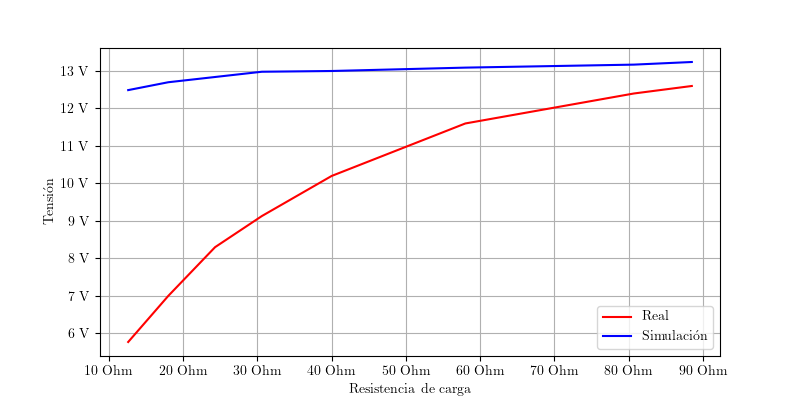
\includegraphics[width=0.8\textwidth]{images/comparacion-general.png}
    \caption{Comparación entre los resultados de las simulaciones y las mediciones realizadas}
    \label{fig:comparacion}
\end{figure}

La diferencia entre la simulación y lo analizado en el marco teórico puede deberse a que, con el objetivo de simplificar el análisis del convertidor forward, se consideró el modelo ideal de todos sus componentes. 
Esto se evidencia en el simulador donde al utilizar modelos reales de los semiconductores la tensión de salida comienza a variar levemente con la carga. 
Las pérdidas en todos los componentes aumentan con la corriente de carga. 
Es por ello que en la práctica los convertidores funcionan a lazo cerrado sensando la tensión o corriente de salida, y por medio de un sistema de realimentación ajustan el ciclo de trabajo para obtener una tensión de salida constante ante los cambios de carga o la tensión de entrada del convertidor.

Si bien en la teoría analizada y en las simulaciones del prototipo los transistores conmutan de forma simultánea, en las mediciones realizadas se aprecia un retardo entre la señal de excitación del MOSFET de lado bajo y la del lado alto. 
Es decir, para la frecuencia de conmutación elegida el transformador del driver no tiene un tiempo despreciable de encendido y apagado como se describió en la nota de aplicación \cite{gatedrivers}.  
En consecuencia, como se observa en la tabla \ref{tab:estados}, se tiene un total de 4 estados en cada ciclo de conmutación:

\begin{table}[H]
    \centering
    \begin{tabular}{ccc}
    \hline
    Estado & MOSFET de lado bajo & MOSFET de lado alto \\ \hline
    1      & OFF                 & OFF                 \\
    2      & ON                  & OFF                 \\
    3      & ON                  & ON                  \\
    4      & OFF                 & ON                  \\ \hline
    \end{tabular}
    \caption{Estados de conmutación del convertidor forward}
    \label{tab:estados}
\end{table}

Se corroboró con el simulador que la tensión a la salida del convertidor se ve afectada por los 2 estados adicionales indeseados a ambos MOSFETs encendidos y ambos MOSFETs apagados.

\begin{table}[H]
    \centering
    \begin{tabular}{lllllll}
    \hline
    $R[\Omega]$ & $I_i[A]$ & $V_o[V]$ & $I_o[A]$ & \multicolumn{1}{c}{$P_i[W]$} & \multicolumn{1}{c}{$P_o[W]$} & \multicolumn{1}{c}{$\eta[\%]$} \\ \hline
    12.6        & 1.46     & 12.49    & 0.99     & 17.65                        & 12.39                        & 70.19                          \\
    18          & 1.33     & 12.70    & 0.71     & 13.72                        & 8.96                         & 65.31                          \\
    24.3        & 1.24     & 12.84    & 0.51     & 10.80                        & 6.60                         & 61.11                          \\
    30.6        & 1.17     & 12.98    & 0.35     & 8.07                         & 4.56                         & 56.51                          \\
    40          & 1.16     & 13.00    & 0.33     & 7.68                         & 4.23                         & 55.08                          \\
    58          & 1.12     & 13.09    & 0.23     & 6.14                         & 2.95                         & 48.05                          \\
    80.7        & 1.10     & 13.17    & 0.16     & 5.11                         & 2.15                         & 42.07                          \\
    88.5        & 1.10     & 13.24    & 0.15     & 4.89                         & 1.95                         & 39.88                          \\ \hline
    \end{tabular}
    \caption{Resultados de las mediciones en la simulación}
    \label{tab:mediciones_sim}
\end{table}